%%%%%%%%%%%%%%%%%%%%%%%%%%%%%%%%%%%%%%%%%%%%%%%%%%%%%%%%%%%%%%%%%%%%%%%%%%%
%
% Template for a LaTex article in English.
%
%%%%%%%%%%%%%%%%%%%%%%%%%%%%%%%%%%%%%%%%%%%%%%%%%%%%%%%%%%%%%%%%%%%%%%%%%%%

\documentclass{article}

% AMS packages:
\usepackage{amsmath, amsthm, amsfonts}
\usepackage{algorithm}
\usepackage[noend]{algpseudocode}
\usepackage{graphicx}
\graphicspath{ {images/} }

% Theorems
%-----------------------------------------------------------------
\newtheorem{thm}{Theorem}[section]
\newtheorem{cor}[thm]{Corollary}
\newtheorem{lem}[thm]{Lemma}
\newtheorem{prop}[thm]{Proposition}
\theoremstyle{definition}
\newtheorem{defn}[thm]{Definition}
\theoremstyle{remark}
\newtheorem{rem}[thm]{Remark}

\makeatletter
\def\BState{\State\hskip-\ALG@thistlm}
\makeatother
%\newcommand*{\rom}[1]{\expandafter\@slowromancap\romannumeral #1@}
\newcommand{\rom}[1]{\uppercase\expandafter{\romannumeral #1\relax}}
% Shortcuts.
% One can define new commands to shorten frequently used
% constructions. As an example, this defines the R and Z used
% for the real and integer numbers.
%-----------------------------------------------------------------
\def\RR{\mathbb{R}}
\def\ZZ{\mathbb{Z}}

% Similarly, one can define commands that take arguments. In this
% example we define a command for the absolute value.
% -----------------------------------------------------------------
\newcommand{\abs}[1]{\left\vert#1\right\vert}

% Operators
% New operators must defined as such to have them typeset
% correctly. As an example we define the Jacobian:
% -----------------------------------------------------------------
\DeclareMathOperator{\Jac}{Jac}

%-----------------------------------------------------------------
\title{Bilateral Normal Filter}
\author{ShengweiZHANG\\
  %% \small Dept. Templates and Editors\\
  %% \small E12345\\
  %% \small Spain
}

\begin{document}
\maketitle

%% \abstract{Compiling Embedded\_thin\_shell progress}
\section{Abstract}
Bilateral filter for processing a normal field defined over an input mesh, smooth the face normal and update the vertexes according the face normal.
\section{The Filter}
\subsection{Normal Filter}
Just directly apply the traditional bilateral filter to the normal field:
\begin{equation}
  n_i' = K_i \sum_{j\in N(i)} \zeta_{ij} W_c(\parallel c_j-c_i\parallel) W_s(\parallel n_j - n_i \parallel) n_j
\end{equation}
where $c_i, n_i$  is the center and normal of face i, $K_i$ is the nomalize factor. $W_c, W_s$ are Guass function, $\zeta_{ij}$ is the weight to account for the influence from surface sampling rate, choose the area $S_j$ of the face j:
\begin{equation}
  \begin{aligned}
    K_i &= \sum_{j\in N(i)} \zeta_{ij} W_c(\parallel c_j-c_i\parallel) W_s(\parallel n_j - n_i \parallel) \\
    W_c(\parallel c_j-c_i \parallel) &= exp(-\frac{(\parallel c_j-c_i \parallel)^2}{2\sigma_c^2})\\
    W_s(\parallel n_j-n_i \parallel) &= exp(-\frac{(\parallel n_j-n_i \parallel)^2} {2\sigma_s^2})\\
    \zeta_{ij} = S_j
  \end{aligned}
\end{equation}
\subsection{Updating Vertexes}
\begin{equation}
  v_i' = v_i + \frac{1}{18} \sum_{v_j \in N_i^v} \sum_{ (v_i, v_j) \in \Delta F_m} n_m'(n_m' \cdot (v_j - v_i))
\end{equation}
\section{Parameter}
The $\sigma_s$'s influence on $W_s$ is:
\begin{equation}
  \begin{aligned}
      W_s(\parallel n_j-n_i \parallel) &= exp(-\frac{(\parallel n_j-n_i \parallel)^2} {2\sigma_s^2})\\
      &= exp(-\frac{n_j^2 + n_i^2  - 2n_jn_i} {2\sigma_s^2}) \\
      &=exp(-\frac{1-cos(\theta)} {\sigma_s^2})
   \end{aligned}
\end{equation}
\begin{figure}[H]
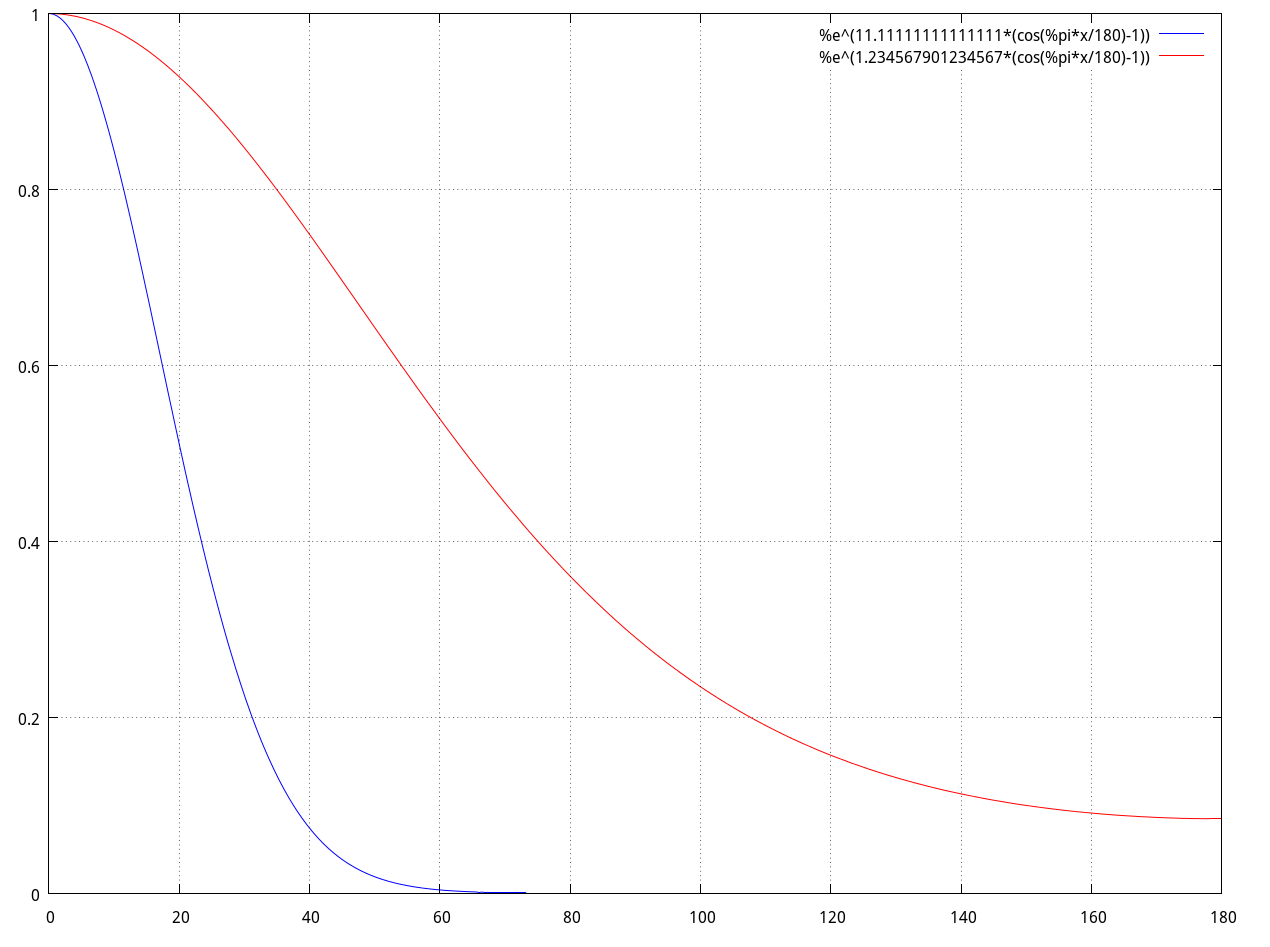
\includegraphics[width=12cm]{theta_inf}
 \caption[The $\sigma_s$'s influence on $W_s$]
   {Blue $\sigma_s$ is 0.3, Red one is 0.9, the horizontal axis is the angle of face normal $n_i$ and $n_j$.}
\centering
\end{figure}
From the Figure 1, as we want to preserve the feature of the model, I set $\sigma_s = 0.3$. For $\sigma_c$ set as the paper's saying: The $\sigma_c$  using the average distance of all adjacent facets in an input mesh generally works the best in our experiments.
\section{Details}
One-ring face $N_{\rom{1}}$ is a set of faces that share edges with $f_i$, and the second type $N_{\rom{2}}$ is a set of faces that common vertices with $f_i$. As the paper's author speculate $N_{\rom{2}}$ is able to better characterize sharp features which is more suitable for CAD-like models. Here I using $N_{\rom{1}}$.
%% \begin{equation}\label{eq:area}
%%   S = \pi r^2
%% \end{equation}
%% One can refer to equations like this: see equation (\ref{eq:area}). One can also
%% refer to sections in the same way: see section \ref{sec:nothing}. Or
%% to the bibliography like this: \cite{Cd94}.

%% \subsection{Subsection}\label{sec:nothing}

%% More text.

%% \subsubsection{Subsubsection}\label{sec:nothing2}

%% More text.

%% % Bibliography
%% %-----------------------------------------------------------------
%% \begin{thebibliography}{99}

%% \bibitem{Cd94} Author, \emph{Title}, Journal/Editor, (year)

%% \end{thebibliography}

\end{document}
